\section{Task and Method}
\label{sec:framework}
\label{sec:framework:problem}

The input is a list of triples $G$, source text $X$, a fixed document ID
$h_0$, and allowed relations $\mathcal R_X$. The list can contain copies
of the same triple. Each relation has at most one nonempty value.
Examples include document fields and receipt fields.
The scorer uses the reference graph $G^*$ to check the output.

The main method has three steps: clean the input, ask a model for a complete
graph, and filter the triples. The prompt can include an error report or
source-line hints. The filter checks each value against the source text.
Reference scores and human review measure output quality.

Figures~\ref{fig:framework_overview} and~\ref{fig:optimization_flow} show a
second path. A learned router gives weights to edits. A selector tries the
edits on graph copies and chooses one at a time.
Section~\ref{sec:impl:optimizer_audit} tests this path with saved proposals.

\begin{figure}[t]
    \centering
    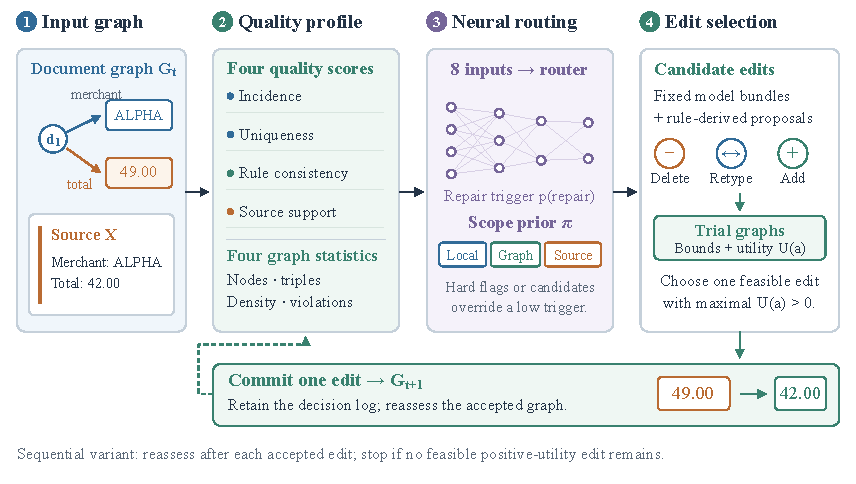
\includegraphics[width=0.98\textwidth]{figure/method/image1.pdf}
    \caption{Repair by choosing edits one at a time. Four quality scores and four
graph counts feed the learned router. It gives a repair score and weights
for three kinds of edits. The selector tries model and rule edits on graph
copies. It applies the allowed edit with the highest positive score, then
checks the graph again. Section~\ref{sec:impl:optimizer_audit} gives this test.}
    \label{fig:framework_overview}
\end{figure}

\subsection{Input Cleanup and Error Report}
\label{sec:framework:profile}

Figure~\ref{fig:scale_relationship} groups the checks into local, graph,
and source checks. They count copies, check the document ID and relation,
and look for the value in the text.

\begin{figure}[t]
    \centering
    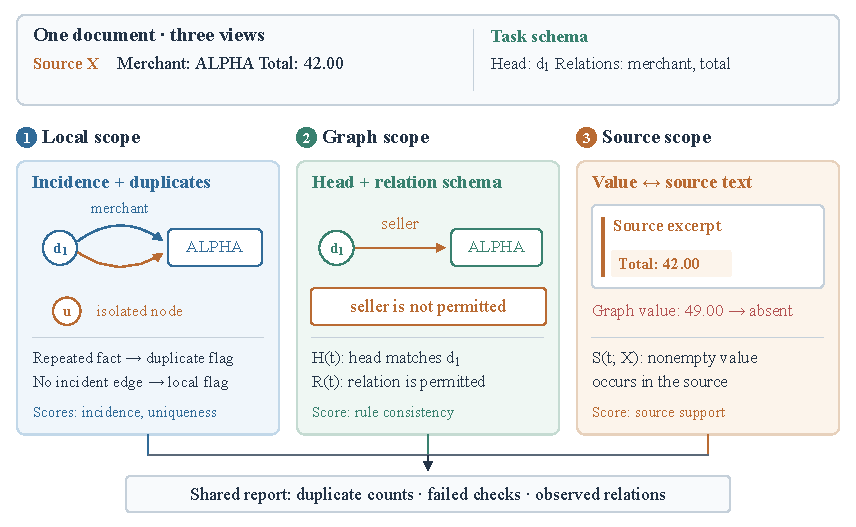
\includegraphics[width=0.98\textwidth]{figure/method/image2.pdf}
    \caption{Three groups of graph checks: repeated facts and unlinked nodes
(local), invalid relations (graph), and values missing from the text
(source). Both repair paths use these groups. Their report follows
Eq.~(\ref{eq:diagnostic_predicates}).}
    \label{fig:scale_relationship}
\end{figure}

The preprocessor $P$ removes duplicate triples. It reverses an edge if its
object is $h_0$ and its subject is a different node. It then removes triples
with an invalid head or relation. Here, the head is the subject of a triple.
The cleaned graph is $G_s=P(G;h_0,\mathcal R_X)$.

For a triple $t=(h,r,o)$, the three checks are
\begin{equation}
    \label{eq:diagnostic_predicates}
    H(t)=\mathbf1[h=h_0],\quad
    R(t)=\mathbf1[r\in\mathcal R_X],\quad
    S(t;X)=\mathbf1[o\ne\emptyset\ \wedge\ o\text{ occurs in }X].
\end{equation}
$H$ checks the document ID, $R$ checks the relation, and $S$ checks whether
the nonempty value occurs in the text.
The error report stores duplicate counts, failed-check positions,
and relations in $G_s$:
\begin{equation}
    \label{eq:diagnostic_context}
    D(G_s,X)=\big(n_{\mathrm{dup}},I_H,I_R,I_S,\mathcal R(G_s)\big).
\end{equation}
For example, $I_S=\{i:S(t_i;X)=0\}$ lists positions that fail the source
check. The report uses the cleaned input. Cleanup removes some errors
before the report is built. We test the effect of adding this report to the
prompt. Fields are optional, and the main method calls the model once for
every document to recover missing values.

\subsection{Generating a Graph from Source Text}
\label{sec:framework:architecture}

The language model returns an ordered list of triples:
\begin{equation}
    \label{eq:proposal_generation}
    C=L_\theta(X,h_0,\mathcal R_X,G_s,D(G_s,X)).
\end{equation}
The prompt asks for a complete graph. It tells the model to copy values from
the text, keep correct fields, and fill missing or wrong values.
The JSON parser returns an empty graph for an invalid response.
Scoring includes these empty graphs. The base prompt uses the same source,
input graph, model settings, and output limit, with the error report removed.

\subsection{Checking the Generated Triples}
\label{sec:framework:constraints}

The gate is a filter. It keeps triples that pass
Eq.~(\ref{eq:diagnostic_predicates}) and keeps at most one value per relation.
Let $\operatorname{uniq}(C)$ remove copies in output order. The triples that
pass the checks are
\begin{equation}
    \label{eq:eligible_candidates}
    C_X=\{t\in\operatorname{uniq}(C):H(t)R(t)S(t;X)=1\}.
\end{equation}
The allowed output sets are
\begin{equation}
    \label{eq:admissible_subsets}
    \mathcal F(C_X)=\left\{A\subseteq C_X:
    \sum_{t\in A}\mathbf1[r_t=r]\leq1,\ \forall r\in\mathcal R_X\right\}.
\end{equation}
The filter scans the triples in order. For each relation, it keeps the first
triple that passes the checks. The output $\widehat G$ has size
\begin{equation}
    \label{eq:selection_size}
    |\widehat G|=\max_{A\in\mathcal F(C_X)}|A|
    =|\{r:\exists t\in C_X,\ r_t=r\}|.
\end{equation}
Each relation forms one group with room for one triple.
The filter keeps one triple from each group that has a valid candidate.
It thus keeps the largest allowed number of candidates.
The first valid value in output order wins when several values pass.

\subsection{Field Meanings and Source Lines}
\label{sec:framework:field_evidence}

A receipt can list a brand name, a company name, a subtotal, and a final
amount. We give each field a short meaning to help the model choose its
value. All receipt repair methods receive these meanings and numbered
source lines.

The source-line index adds hints for each field. Fixed patterns find company
terms, address terms, postcodes, dates, and total labels. Each matching line
is an anchor. The index includes that line, one line before it, and two
lines after it. Simple receives the full source and field meanings.
Evidence Index also receives the line hints.

The receipt filter uses the same whitespace rule as the parser.
$N(s)$ changes each run of spaces or line breaks to one space and trims the
ends. The source check is
\begin{equation}
    S_{\mathrm{ws}}(t;X)=\mathbf1[|N(o)|>0\ \wedge\
    N(o)\text{ occurs in }N(X)].
\end{equation}
It keeps word boundaries, case, and punctuation. The receipt follow-up uses
this check. Earlier tests use the original exact-text check.
